\documentclass{article}

\usepackage{graphicx}
\usepackage{tikz}
\usepackage{tikzsymbols}
\usetikzlibrary{calc,patterns,shapes.geometric}
\pagestyle{empty}
\usepackage[margin=0pt]{geometry}
\geometry{papersize={14in,12in}}

\def\centerarc[#1](#2)(#3:#4:#5){\draw[#1] ($(#2)+({#5*cos(#3)},{#5*sin(#3)})$) arc (#3:#4:#5);}

\begin{document}
	\begin{figure}
		\centering
		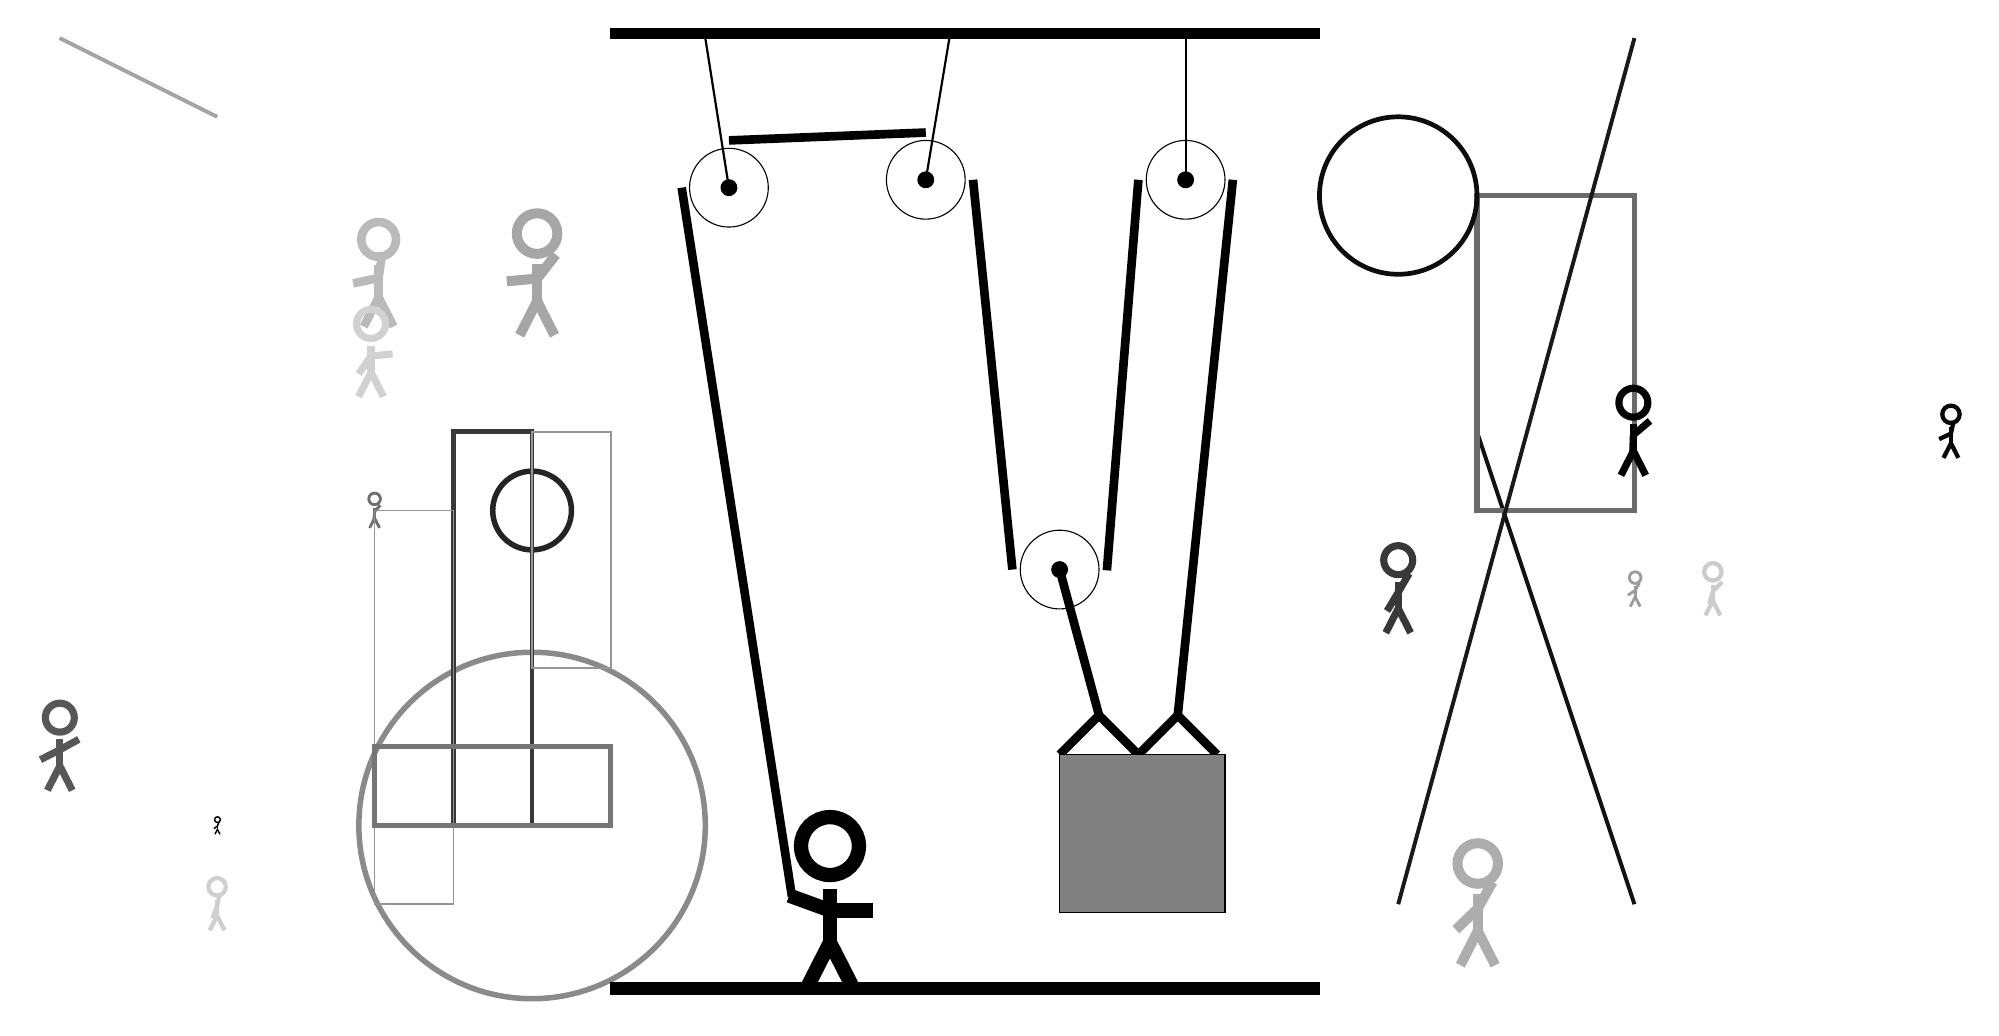
\begin{tikzpicture}
			%%%%% START %%%%%
			
			\draw[fill=black] (-3, 9) rectangle (6, 9.125);
			
			\draw (1, 7.2) circle (0.5);
			\draw[fill=black] (1, 7.2) circle (0.1);
			\draw[thick] (1, 7.2) -- (1.3, 9);
			
			\draw (4.3, 7.2) circle (0.5);
			\draw[fill=black] (4.3, 7.2) circle (0.1);
			\draw[thick] (4.3, 7.2) -- (4.3, 9);
			
			\draw (2.7, 2.25) circle (0.5);
			\draw[fill=black] (2.7, 2.25) circle (0.1);
			
			\draw[line width=1.1mm]  (2.7, -0.1) -- (3.2, 0.4) -- (3.7, -0.1) -- (4.2, 0.4) -- (4.7, -0.1);
			\draw[fill=black!50] (2.7, -0.1) rectangle (4.8, -2.1);
			
			\draw (-1.5, 7.1) circle (0.5);
			\draw[fill=black] (-1.5, 7.1) circle (0.1);
			\draw[thick] (-1.5, 7.1) -- (-1.8, 9);
			
			\draw[line width=1.1mm](-0.7, -1.9) --  (-2.1, 7.1);
			\centerarc[line width=1.1mm](-1.5, 7.1)(90:180:0.6);
			\draw[line width=1.1mm](-1.5, 7.7) -- (1, 7.8);
			\centerarc[line width=1.1mm](1, 7.2)(0:90:0.6);
			\draw[line width=1.1mm](1.6, 7.2) -- (2.1, 2.25);
			\centerarc[line width=1.1mm](2.7, 2.25)(180:370:0.6);
			\draw[line width=1.1mm] (3.3, 2.24) -- (3.7, 7.2);
			\centerarc[line width=1.1mm](4.3, 7.2)(0:180:0.6);
			\draw[line width=1.1mm](4.2, 0.4) -- (4.9, 7.2);
			\draw[line width=1.1mm] (3.2, 0.4) -- (2.7, 2.25);
			
			\node at (-0.2, -2) {\Strichmaxerl[10][-20][0]};
			
			\draw [line width=0.7mm, color=black!86](-4, 3) circle (0.5);
			
			\draw [line width=0.7mm, color=black!46](-4, -1) circle (2.2);
			\node[line width=0.7mm, color=black!27] at (-6, 6) {\Strichmaxerl[6][12][82]};
			\draw[line width=0.6mm, color=black!78] (-5, -1) rectangle (-4, 4);
			\node[line width=0.3mm, color=black!18] at (-6, 5) {\Strichmaxerl[5][55][6]};
			
			\draw[line width=0.5mm, color=black!93](10, -2) -- (8, 4);
			\node[line width=0.3mm, color=black!100] at (-8, -1) {\Strichmaxerl[1][35][69]};
			
			\node[line width=0.6mm, color=black!32] at (8, -2) {\Strichmaxerl[7][44][61]};
			\node[line width=0.6mm, color=black!20] at (11, 2) {\Strichmaxerl[3][74][44]};
			
			\node[line width=0.5mm, color=black!35] at (-4, 6) {\Strichmaxerl[7][5][52]};
			\node[line width=0.6mm, color=black!57] at (-6, 3) {\Strichmaxerl[2][85][49]};
			\node[line width=0.7mm, color=black!39] at (10, 2) {\Strichmaxerl[2][33][61]};
			\draw[line width=0.2mm, color=black!41] (-3, 4) rectangle (-4, 1);
			
			\draw[line width=0.7mm, color=black!58] (8, 7) rectangle (10, 3);
			\draw[line width=0.5mm, color=black!36](-8, 8) -- (-10, 9);
			\draw[line width=0.2mm, color=black!42] (-5, 3) rectangle (-6, -2);
			
			\node[line width=0.6mm, color=black!19] at (-8, -2) {\Strichmaxerl[3][69][78]};
			\node[line width=0.3mm, color=black!66] at (-10, 0) {\Strichmaxerl[5][27][29]};
			\draw [line width=0.6mm, color=black!95](7, 7) circle (1.0);
			
			\node[line width=0.4mm, color=black!78] at (7, 2) {\Strichmaxerl[5][59][60]};
			\draw[line width=0.5mm, color=black!90](7, -2) -- (10, 9);
			\node[line width=0.6mm, color=black!99] at (10, 4) {\Strichmaxerl[5][88][40]};
			
			\draw[line width=0.6mm, color=black!54] (-3, 0) rectangle (-6, -1);
			\node[line width=0.7mm, color=black!97] at (14, 4) {\Strichmaxerl[3][25][78]};
			
			\draw[fill=black] (-3, -3) rectangle (6, -3.15);
			
			%%%%% END %%%%%
		\end{tikzpicture}
	\end{figure}	
\end{document}